% Author: Alfredo Sánchez Alberca (asalber@ceu.es)
\chapter{Derivadas de funciones de varias variables}

\section{Fundamentos teóricos}
El concepto de derivada es uno de los más importantes del Cálculo
pues resulta de gran utilidad en el estudio de funciones y tiene
multitud de aplicaciones. En esta práctica introducimos este
concepto de derivada parcial en funciones de varias variables y presentamos algunas de sus aplicaciones.

\subsection{Derivadas parciales de una función de $n$ variables}
Recordemos que la derivada de una función de una única variable en
un punto $x=a$ se define como la tasa de variación instantánea de la
función en dicho punto. Si llamamos $h$ al incremento en la
variable, la derivada de la función en $x=a$ se nota como $f'(a)$ ó
$\dfrac{{df}} {{dx}}(a)$, y se calcula como:

\[
f'(a) = \frac{df}{dx}(a) = \mathop {\lim
}\limits_{h \to 0} \frac{{f(a + h) - f(a)}} {h}
\]

Y, en general, para cualquier $x$ en un conjunto en el que la
función de una única variable sea derivable, puede definirse la
función derivada $f'(x)$ ó $\dfrac{df}{dx}$,
mediante el límite:

\[
f'(x) = \frac{df}{dx} = \mathop {\lim }\limits_{h
\to 0} \frac{{f(x + h) - f(x)}} {h}
\]
que, no obstante, se calcula aplicando las adecuadas reglas de
derivación, más bien que acudiendo a la resolución directa del
límite.

De igual forma, si tenemos una función de $n$ variables
$f(\vec{x})=f(x_1,x_2,...,x_n)$, se pueden definir esas mismas tasas
de variación instantáneas con respecto a cada una de las variables
en un punto $\vec{a}=(a_1,a_2,...,a_n)$, para obtener las
\emph{Derivadas Parciales} de la función con respecto a cada una de
las variables en el punto $\vec{x}=\vec{a}$, que se notarán como
$f_{x_i}(\vec{a})$, o bien por $\dfrac{\partial f}{\partial
x_i}(\vec{a})$:

\[
f_{x_i}(\vec{a})=\dfrac{\partial f}{\partial
x_i}(\vec{a})=\lim_{h\rightarrow
0}\frac{f(a_1,\ldots,a_i+h,\ldots,a_n)-f(a_1,\ldots,a_i,\ldots,a_n)}{h},
\]

Y la \emph{Función Derivada Parcial} con respecto a cualquiera de
las variables $x_i$, para todos los $\vec{x}$ de un conjunto, que se
notará como $f_{x_i}$, o $\dfrac{\partial f}{\partial x_i}$:

\[
f_{x_i}=\dfrac{\partial f}{\partial x_i}=\lim_{h\rightarrow
0}\frac{f(x_1,\ldots,x_i+h,\ldots,x_n)-f(x_1,\ldots,x_i,\ldots,x_n)}{h},
\]

Lo cual, a efectos de cálculo, se resume en que la derivada parcial
de una función de varias variables se obtiene como la derivada de
una función de una única variable, que es aquella con respecto a la
que se deriva, y constantes el resto. Como consecuencia, las reglas
de derivación también se aplican en el cálculo de las derivadas
parciales de este tipo de funciones, sin más que considerar
constantes todas las variables con respecto a las que no estamos
derivando.

Si para las funciones de una variable la derivada en un punto $a$
tiene una interpretación gráfica sencilla como la pendiente de la
recta tangente a la gráfica de la función en el punto $(a,f(a))$,
también para funciones de dos variables la derivada parcial con
respecto a $x$ en el punto $\vec{a}=(x_0,y_0)$:

\[
\frac{{\partial f}} {{\partial x}}(x_0 ,y_0 ) = \mathop {\lim
}\limits_{h \to 0} \frac{{f(x_0  + h,y_0 ) - f(x_0 ,y_0 )}} {h}
\]
representa la pendiente de la recta tangente a la curva que se
obtiene al cortar la gráfica de la función en el punto
$(x_0,y_0,z_0=f(x_0,y_0))$ mediante el plano en el que $y$ permanece
constante e igual a $y_0$, y tan sólo varía el valor de $x$. E
igualmente, la derivada parcial con respecto a $y$ será la pendiente
de la recta tangente a la curva que se obtiene al cortar la gráfica
de la función en $(x_0,y_0,z_0=f(x_0,y_0))$ mediante el plano
$x=x_0$.

\begin{figure}[h!]
\begin{center}
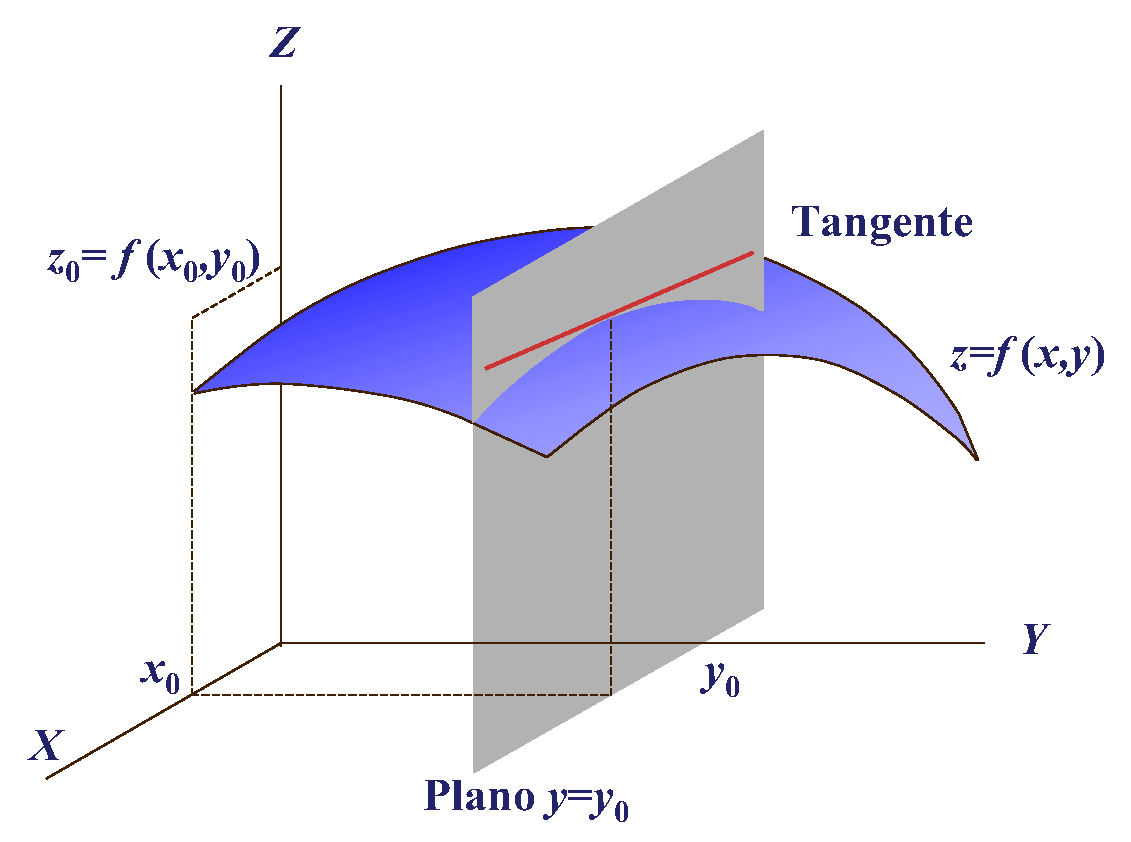
\includegraphics[scale=0.4]{img/derivadas_varias_variables/tangentesuperficie}
\caption{La derivada parcial de una función $f(x,y)$ con respecto a
$x$ en el punto $(x_0,y_0)$, como la pendiente de la recta tangente
a la curva descrita por la intersección de la superficie de $f$ y el
plano de ecuación $y=y_0$.}
\end{center}
\end{figure}


\subsection{Derivadas parciales sucesivas de una función de $n$
variables}

De la misma forma que en las funciones de una variable, mediante los
límites que las definen, siempre y cuando existan, obtenemos las
segundas, terceras y derivadas de cualquier orden. Es decir, si $f$
es una función real de $n$ variables, con sus correspondientes
derivadas parciales, a su vez también las mismas son funciones de
$n$ variables que, en determinadas condiciones, podrán derivarse de
nuevo con respecto a sus $n$ variables para obtener derivadas
parciales segundas, y así sucesivamente hasta órdenes superiores de
derivación.

Para la derivada parcial de segundo orden se utiliza la notación
$f_{x_ix_j}$ ó $\dfrac{{\partial ^2 f}} {{\partial x_j \partial x_i
}}$:


\[
f_{x_i x_j }  = \frac{{\partial ^2 f}} {{\partial x_j \partial x_i
}} = \frac{\partial } {{\partial x_j }}\left( {\frac{{\partial f}}
{{\partial x_i }}} \right)
\]

Por ejemplo, para una función de dos variables $f(x,y)$, tenemos dos derivadas parciales de primer orden, que siguen
siendo funciones de las variables $x$ e $y$:
\[
\frac{\partial f}{\partial x}(x,y)\qquad \frac{\partial f}{\partial y}(x,y) 
\] y cuatro diferentes de segundo orden, que también serán funciones de $x$ e $y$, aunque ya no se
refleje para aligerar la notación:
\[
\frac{\partial}{\partial x}\left({\frac{\partial f}{\partial x}}\right) = \frac{\partial^2 f}{\partial x^2}
\]
\[
\frac{\partial}{\partial y}\left({\frac{\partial f}{\partial x}}\right) = \frac{\partial^2 f}{\partial y\partial x}
\]
\[
\frac{\partial}{\partial x}\left({\frac{\partial f}{\partial y}}\right) = \frac{\partial^2 f}{\partial x\partial y}
\]
\[
\frac{\partial}{\partial y}\left({\frac{\partial f}{\partial y}}\right) = \frac{\partial^2 f}{\partial y^2}
\]

La primera y la última reciben el nombre de derivadas segundas, mientras que la segunda y tercera se denominan derivadas
cruzadas.

Si procedemos con las derivadas parciales de tercer orden tendríamos ocho diferentes, y el número es más amplio con
funciones de tres o más variables.
No obstante, el teorema conocido con \emph{Teorema de Schwartz de las Derivadas Cruzadas} reduce el número de derivadas
parciales diferentes:

\begin{teorema}[Schwartz]
Si $f$ es una función de $n$ variables con derivadas parciales segundas cruzadas continuas en un conjunto abierto que
contiene al punto $a$, entonces en dicho punto se cumple
\[
\frac{\partial ^2 f}{\partial x_i \partial x_j } = \frac{\partial ^2 f}{\partial x_j \partial x_i }
\] 
e igual con las derivadas cruzadas de tercer y superior orden.
\end{teorema}

Es decir, si se cumplen las hipótesis del teorema de Schwartz concluimos que, a efectos de cálculo, tan sólo importa el
número de veces que se deriva respecto a cada variable, pero no el orden de la derivación.

\subsection{Vector gradiente y matriz hessiana}
A partir de las derivadas parciales de primer orden de un campo escalar, podemos definir el siguiente vector:

\begin{definicion}[Vector gradiente]
Dado un campo escalar $f(x_1,\ldots,x_n)$, se llama \emph{gradiente} de $f$, y se escribe $\nabla f$, a la función que a
cada punto $a=(a_1,\ldots,a_n)$ le asigna el vector cuyas coordenadas cartesianas son las derivadas parciales de $f$ en
$a$,
\[
\nabla f(a)=\left(\frac{\partial f}{\partial x_1}(a),\ldots,\frac{\partial f}{\partial x_n}(a)\right).
\]
\end{definicion}

El vector gradiente en un punto dado tiene la misma magnitud y dirección que la velocidad máxima de variación de la
función en ese punto, por lo que $\nabla f(a)$ indica la dirección de máximo crecimiento de $f$ en el punto $a$,
mientras que $-\nabla f(a)$ indica la dirección de máximo decrecimiento.

Y a partir de las derivadas parciales de segundo orden, podemos definir la siguiente matriz:

\begin{definicion}[Matriz hessiana]
Dada una función de varias variables $f(x_1,\ldots,x_n)$, para la que existen todas sus derivadas parciales de segundo
orden en un punto $a=(a_1,\ldots,a_n)$, se define la \emph{matriz hessiana} de $f$ en $a$, y se nota $\nabla^2f(a)$, como la
matriz cuadrada cuyos elementos son
\[
\nabla^2f(a)=\left(
\begin{array}{cccc}
\dfrac{\partial^2 f}{\partial x_1^2}(a) & 
\dfrac{\partial^2 f}{\partial x_1 \partial x_2}(a) &
\cdots &
\dfrac{\partial^2 f}{\partial x_1 \partial x_n}(a)\\
\dfrac{\partial^2 f}{\partial x_2 \partial x_1}(a) &
\dfrac{\partial^2 f}{\partial x_2^2}(a) & 
\cdots &
\dfrac{\partial^2 f}{\partial x_2 \partial x_n}(a)\\
\vdots & \vdots & \ddots & \vdots \\
\dfrac{\partial^2 f}{\partial x_n \partial x_1}(a) &
\dfrac{\partial^2 f}{\partial x_n \partial x_2}(a) &
\cdots &
\dfrac{\partial^2 f}{\partial x_n^2}(a)
\end{array}
\right).
\]
Al determinante de esta matriz se le llama \emph{hessiano} de $f$ en $a$, y se nota $Hf(a)=|\nabla^2f(a)|$.
\end{definicion}

Entre las utilidades de la matriz Hessiana y el hessiano está la determinación de los extremos relativos y los puntos de
silla de una función. 

\subsection{Derivada direccional}
Ya se ha visto que la derivadas parciales miden la tasa de variación instantánea de la función con respecto a cada uno
de sus variables, es decir, en la dirección de cada uno de los ejes de coordenadas. 
Pero, \emph {¿qué pasa si nos movemos en cualquier otra dirección?}
La tasa de variación instantánea de $f$ en un punto $a$ en la dirección de un vector unitario cualquiera $u$ se conoce
como \emph{derivada direccional}.

\begin{definicion}[Derivada direccional]
Dado un campo escalar $f$ de $\mathbb{R}^n$, un punto $a$ y un vector unitario $\mathbf{u}$ en ese espacio, el límite
\[
f'_{\mathbf{u}}(a) = \lim_{h\rightarrow 0}\frac{f(a+h\mathbf{u})-f(a)}{h},
\] 
cuando existe, se llama \emph{derivada direccional} de $f$ en el punto $a$ en la dirección de $\mathbf{u}$.
\end{definicion}
Se cumple 
\[
f'_{\mathbf{u}}(a) =\nabla f(a)\cdot \mathbf{u}.
\]
Obsérvese que las derivadas parciales son las derivadas direccionales en las direcciones de los vectores coordenados.

\subsection{Derivación implícita}
Si se sabe que la ecuación 
\[
f(x,y)=0
\]
define a $y$ como función de $x$, $y=h(x)$, alrededor de cierto valor $x=x_0$ para el que $y=h(x_0)=y_0$, entonces, si se toma la trayectoria $g(x)=(x,h(x))$, la ecuación anterior se puede expresar como
\[
(f\circ g)(x) = f(g(x)) = f(x,h(x))=0,
\]
de modo que usando la regla de la cadena sobre se tiene
\[
(f\circ g)'(x) = \nabla f(g(x))\cdot g'(x) = \left(\frac{\partial f}{\partial x}, \frac{\partial f}{\partial y}\right)\cdot (1,h'(x)) = 
\frac{\partial f}{\partial x}+\frac{\partial f}{\partial y}h'(x) = 0,
\] 
de donde se deduce
\[
y'=h'(x)=\frac{-\dfrac{\partial f}{\partial x}}{\dfrac{\partial f}{\partial y}}
\]

\subsection{Cálculo de extremos}
Si $a$ es un extremo de un campo escalar $f$ de $\mathbb{R}^n$, entonces se cumple que $a$ es un punto crítico de $f$,
es decir,
\[
\nabla f(P) = 0,
\]
Sin embargo, no todos los puntos críticos son extremos relativos. 
Existen puntos como el de la figura~\ref{g:punto_silla} donde se anula el gradiente y que no son puntos de máximo, ni de
mínimo.
Estos puntos se conocen como \emph{puntos de silla}. 
\begin{figure}[htp]
\begin{center}
\scalebox{1}{\psset{unit=0.65}
\psset{viewpoint=50 50 30 rtp2xyz,Decran=50}
\begin{pspicture*}(-7,-4.2)(7,4.3)
%\psSolid[object=grille,base=-4 4 -4 4,action=draw]
\psSurface[fillcolor=blue!50,ngrid=.25 .25,incolor=yellow,algebraic,linewidth=0.25\pslinewidth,linecolor=gray](-2,-2)(2,2){x^2-y^2}
\axesIIID(1,0,0)(4,4,4)
\psPoint(0,0,0){p}
\psdots[linecolor=red](p)
\uput[r](p){$(0,0,0)$ Punto de silla}
\end{pspicture*}}.
\caption{Gráfica de la función $f(x,y)=x^2-y^2$, que tiene un punto de silla en $(0,0)$. }
\label{g:punto_silla}
\end{center}
\end{figure}

Afortunadamente, es posible determinar si un punto crítico es un extremo relativo o un punto de silla a partir de la
matriz Hessiana y el hessiano. 

\begin{teorema}
Dado un punto crítico $a$ de un campo escalar $f$ que tiene matríz hessiana $Hf(a)$, se cumple
\begin{itemize}
\item Si $\nabla^2f(a)$ es definido positivo entonces $f$ tiene un mínimo relativo en $a$.
\item Si $\nabla^2f(a)$ es definido negativo entonces $f$ tiene un máximo relativo en $a$.
\item Si $\nabla^2f(a)$ es indefinido entonces $f$ tiene un punto de silla en $a$.
\end{itemize}
\end{teorema}
En el caso de que $\nabla^2f(a)$ sea semidefinido, no se puede obtener ninguna conclusión y hay que recurrir a derivadas
parciales de orden superior.

En el caso particular de un campo escalar de dos variables se tiene
\begin{teorema}
Dado un punto crítico $a=(x_0,y_0)$ de un campo escalar $f(x,y)$ que tiene matríz hessiana $\nabla^2f(a)$, se cumple
\begin{itemize}
\item Si $Hf(a)>0$ y $\dfrac{\partial^2 f}{\partial x^2}(a)>0$ entonces $f$ tiene un mínimo relativo en $a$.
\item Si $Hf(a)>0$ y $\dfrac{\partial^2 f}{\partial x^2}(a)<0$ entonces $f$ tiene un máximo relativo en $a$.
\item Si $Hf(a)<0$ entonces $f$ tiene un punto de silla en $a$.
\end{itemize}
\end{teorema}

\newpage

\section{Ejercicios resueltos}
\begin{enumerate}[leftmargin=*]
\item Calcular la recta tangente y el plano normal a la trayectoria
\[
f(t)=
\begin{cases}
x=\sin(t),\\
y=\cos(t),\\
z=\sqrt(t),
\end{cases}
\quad t\in \mathbb{R};
\] 
en el instante $t=1$ y dibujarlos.
  
\begin{indicacion}
Para dibujar la trayectoria:
\begin{enumerate}
\item Definir la función introduciendo la expresión \comando{f(t):=[sin(t),cos(t),sqrt(t)]} en la ventana de Álgebra.
\item Abrir una nueva venta gráfica en 3D con el menú \menu{Ventana > Nueva Ventana 3D} y seleccionar el menú \menu{Ventana > Mosaico Vertical} para ver al mismo tiempo la venta de Álgebra y la ventana gráfica.
\item Hacer clic en el botón \boton{Representar} de la ventana gráfica.
\end{enumerate}
Para calcular la recta tangente y dibujar su gráfica:
\begin{enumerate}
\item Introducir la expresión \comando{f(1)} en la ventana de Álgebra.
\item Hacer clic en el botón \boton{Representar} de la ventana gráfica.
\item Introducir la expresión \comando{f(1)+tf'(1)} en la ventana de Álgebra y hacer clic en el botón \boton{Simplificar}.
\item Hacer clic en el botón \boton{Representar} de la ventana gráfica.
\end{enumerate}
Para calcular el plano normal y dibujar su gráfica:
\begin{enumerate}
\item Introducir la expresión \comando{([x,y,z]-f(1))f'(1)=0} en la ventana de Álgebra y hacer clic en el botón \boton{Simplificar}.
\item Hacer clic en el botón \boton{Representar} de la ventana gráfica.
\end{enumerate}
\end{indicacion}    
  
\item Dada la función $f(x,y)=y^2-x^2$, se pide:
\begin{enumerate}
\item Dibujar su gráfica. 
\begin{indicacion}
\begin{enumerate}
\item Introducir la expresión \comando{f(x,y):=y\^{}2-x\^{}2}.
\item Hacer clic sobre el botón \boton{Ventana 3D} para pasar a la ventana de gráficas 3D.
\item Hacer clic sobre el botón \boton{Representar}).
\end{enumerate}
\end{indicacion}

% \item Dibujar las curvas de nivel $f(x,y)=k$, para valores enteros de $k$ desde 1 hasta 5.
% \begin{indicacion}
% \begin{enumerate}
% \item Introducir la ecuación \comando{f(x,y)=k} para cada valor de $k$.
% \item Hacer clic sobre el botón \boton{Ventana 2D} para pasar a la ventana de gráficas 2D.
% \item Hacer clic sobre el botón \boton{Representar Expresión}).
% \end{enumerate}
% \end{indicacion}

\item Dibujar el plano $x=1$. ¿Qué figura forma la intersección de este plano con la gráfica de $f$?
\begin{indicacion}
\begin{enumerate}
\item Introducir la ecuación del plano \comando{x=1}.
\item Hacer clic sobre el botón \boton{Ventana 3D} para pasar a la ventana de gráficas 3D.
\item Hacer clic sobre el botón \boton{Representar}).
\end{enumerate}
\end{indicacion}

\item Calcular la derivada de $f(1,y)$ en $y=2$.
\begin{indicacion}
\begin{enumerate}
\item Introducir la expresión \comando{f(1,y)}.
\item Hacer clic sobre el botón \boton{Hallar una derivada}.
\item En el cuadro de diálogo que aparece, hacer clic en el botón \boton{Simplificar}.
\item Hacer clic sobre el botón \boton{Sustituir variables}.
\item En el cuadro de diálogo que aparece introducir el valor 2 y hacer clic en el botón \boton{Simplificar}.
\end{enumerate}
\end{indicacion}

\item Dibujar el plano $y=2$. ¿Qué figura forma la intersección de este plano con la gráfica de $f$?
\begin{indicacion}
\begin{enumerate}
\item Introducir la ecuación del plano.
\item Hacer clic sobre el botón \boton{Ventana 3D} para pasar a la ventana de gráficas 3D.
\item Hacer clic sobre el botón \boton{Representar}).
\end{enumerate}
\end{indicacion}

\item Calcular la derivada de $f(x,2)$ en $x=1$.
\begin{indicacion}
\begin{enumerate}
\item Introducir la expresión \comando{f(x,2)}.
\item Hacer clic sobre el botón \boton{Hallar una derivada}.
\item En el cuadro de diálogo que aparece, hacer clic en el botón \boton{Simplificar}.
\item Hacer clic sobre el botón \boton{Sustituir variables}.
\item En el cuadro de diálogo que aparece introducir el valor 1 y hacer clic en el botón \boton{Simplificar}.
\end{enumerate}
\end{indicacion}

\item Calcular la derivadas parciales de $f$ en el punto $(1,2)$. ¿Qué conclusiones sacas?
\begin{indicacion}
\begin{enumerate}
\item Introducir la expresión \comando{f(x,y)} o seleccionarla en la expresión anterior. 
\item Hacer clic sobre el botón \boton{Hallar una derivada}.
\item En el cuadro de diálogo que aparece, hacer clic en el botón \boton{Simplificar}.
\item Hacer clic sobre el botón \boton{Sustituir variables}.
\item En el cuadro de diálogo que aparece introducir el valor 1 y hacer clic en el botón \boton{Simplificar}.
\end{enumerate}
\end{indicacion}
\end{enumerate}


\item  Calcular las siguientes derivadas parciales:
\begin{enumerate}
\item  $\dfrac{\partial }{\partial V}\dfrac{nRT}{V}.$

\begin{indicacion}
Introducir la expresión \comando{DIF(nRT/V, V)} en la ventana de Álgebra y hacer clic en el botón \boton{Simplicar}.
\end{indicacion}

\item  $\dfrac{\partial ^{2}}{\partial x\partial y}e^{x+y}\sen(x/y).$
\begin{indicacion}
Introducir la expresión \comando{DIF(DIF(exp(x+y)sin(x/y), y), x)} en la ventana de Álgebra y hacer clic en el botón \boton{Simplicar}.
\end{indicacion}
\end{enumerate}

\item Dada la función $f(x,y)=20-4x^2-y^2$, se pide calcular en el punto $(2,-3)$:
\begin{enumerate}
\item Vector gradiente.
\begin{indicacion}
\begin{enumerate}
\item Definir la función introduciendo la expresión \comando{f(x,y):=20-4x\^{}2-y\^{}2}.
\item Introducir la expresión \comando{f'(2,-3)}.
\item Hacer clic en el botón \boton{Simplificar}.
\end{enumerate}
\end{indicacion}

\item Matriz hessiana.
\begin{indicacion}
\begin{enumerate}
\item Introducir la expresión \comando{f''(2,-3)}.
\item Hacer clic en el botón \boton{Simplificar}.
\end{enumerate}
\end{indicacion}

\item Calcular el determinante hessiano.
\begin{indicacion}
\begin{enumerate}
\item Introducir la expresión \comando{DET(f''(2,-3))}.
\item Hacer clic sobre el botón \boton{Simplificar}.
\end{enumerate}
\end{indicacion}
\end{enumerate} 


% \item Dada la función
% \[
% f(x,y,z)=\sen((x^2-y^2)z)
% \]
% \begin{enumerate}
% \item Definir la función.
% \begin{indicacion}
% Introducir la expresión \comando{f(x,y,z):=sin((x\^{}2-y\^{}2)z)}.
% \end{indicacion}
% 
% \item Calcular su vector gradiente en el punto $(0,-1,\pi/2)$.
% \begin{indicacion}
% \begin{enumerate}
% \item Introducir la expresión \comando{f'(0,-1,pi/2)}.
% \item Hacer clic sobre el botón \boton{Simplificar}.
% \end{enumerate}
% \end{indicacion}
% 
% \item Calcular su matriz Hessiana en el punto $(0,-1,\pi/2)$.
% \begin{indicacion}
% \begin{enumerate}
% \item Introducir la expresión \comando{f''(0,-1,pi/2)}.
% \item Hacer clic sobre el botón \boton{Simplificar}.
% \end{enumerate}
% \end{indicacion}
% 
% \item Comprobar que se cumple el teorema Schwartz de las derivadas para las derivas cruzadas:
% \begin{enumerate}
% \item $\dfrac{{\partial ^3 f}} {{\partial x\partial z\partial y}}$
% \begin{indicacion}
% \begin{enumerate}
% \item Introducir la expresión \comando{f(x,y,z)}.
% \item Hacer clic sobre el botón \boton{Hallar una derivada}.
% \item En el cuadro de diálogo que aparece seleccionar la variable $y$ y hacer clic en el botón \boton{Simplificar}.
% \item Repetir el proceso con la expresión resultante, seleccionando esta vez la variables $z$.
% \item Repetir una vez más el proceso con la expresión resultante, seleccionando esta vez la variables $x$.
% \end{enumerate}
% \end{indicacion}
% 
% \item $\dfrac{{\partial ^3 f}} {{\partial z\partial x\partial y}}$
% \begin{indicacion}
% \begin{enumerate}
% \item Introducir la expresión \comando{f(x,y,z)}.
% \item Hacer clic sobre el botón \boton{Hallar una derivada}.
% \item En el cuadro de diálogo que aparece seleccionar la variable $y$ y hacer clic en el botón \boton{Simplificar}.
% \item Repetir el proceso con la expresión resultante, seleccionando esta vez la variables $x$.
% \item Repetir una vez más el proceso con la expresión resultante, seleccionando esta vez la variables $z$.
% \end{enumerate}
% \end{indicacion}
% \end{enumerate}
% 
% ¿Puedes predecir el valor de $\dfrac{{\partial ^3 f}} {{\partial y\partial x\partial z}}$?
% \end{enumerate}

\item Hallar la recta normal y el plano tangente a la superficie $S: x+2y-\log z +4 =0$ en el punto $(0,-2,1)$ y dibujarlos.
\begin{indicacion}
Para dibujar la gráfica de la superficie:
\begin{enumerate}
\item Definir la función introduciendo la expresión \comando{f(x,y,z):=x+2y-log(z)+4} en la ventana de Álgebra.
\item Introducir la expresión \comando{f(x,y,z)=0} en la ventana de Álgebra.
\item Seleccionar el menú \menu{Resolver > Expresión}.
\item En el cuadro de diálogo que aparece seleccionar la variable \opcion{z} en la lista \campo{Variables}, marcar la opción \opcion{Real} en el campo \campo{Dominio} y hacer clic en el botón \boton{Resolver}.
\item Hacer clic en el botón \boton{Ventana 3D} para pasar a la ventana gráfica 3D.
\item Hacer clic en el botón \boton{Representar}.
\end{enumerate}
Para dibujar la gráfica de la recta normal:
\begin{enumerate}[resume]
\item Hacer clic en el botón \boton{Activar la ventana de Álgebra} para pasar a la ventana de expresiones.
\item Introducir la expresión \comando{}
\item Introducir la expresión \comando{[0,-2,1]+tf'(0,-2,1)}.
\item Hacer clic en botón \boton{Simplificar}.
\item Hacer clic en el botón \boton{Ventana 3D} para pasar a la ventana gŕafica 3D.
\item Hacer clic en el botón \boton{Representar}.
\end{enumerate}
Para dibujar el plano tangente:
\begin{enumerate}[resume]
\item Introducir la expresión \comando{([x,y,z]-[0,-2,1])f'(0,-2,1)=0}.
\item Hacer clic en botón \boton{Simplificar}.
\item Hacer clic en el botón \boton{Ventana 3D} para pasar a la ventana gŕafica 3D.
\item Hacer clic en el botón \boton{Representar}.
\end{enumerate}
\end{indicacion}

% \item La ecuación $x+y-2e^y+2=0$ define implícitamente una función $y=f(x)$ alrededor del punto $(0,0)$. Calcular
% $f'(0)$.
% \begin{indicacion}
% \begin{enumerate}
% \item Introducir la expresión \comando{x+y-2\#e\^{}y+2}.
% \item Hacer clic sobre el botón \boton{Hallar una derivada}.
% \item En el cuadro de diálogo que aparece seleccionar la variable $x$ y hacer clic en el botón \boton{Simplificar}. 
% \item Seleccionar de nuevo la expresión inicial.
% \item Hacer clic sobre el botón \boton{Hallar una derivada}.
% \item En el cuadro de diálogo que aparece seleccionar la variable $y$ y hacer clic en el botón \boton{Simplificar}.
% \item Introducir la expresión \comando{-\#i/\#j} donde \comando{\#i} es la etiqueta de la expresión de la derivada
% parcial con respecto a $x$ y \comando{\#j} es la etiqueta de la expresión de la derivada parcial con respecto a $y$.
% \item Hacer clic sobre el botón \boton{Sustituir}.
% \item En el cuadro de diálogo que aparece, seleccionar $x$ e introducir el valor $0$, seleccionar $y$ e
% introducir el valor $0$, y hacer clic en el botón \boton{Simplificar}.
% \end{enumerate}
% \end{indicacion}

\item Calcular la derivada direccional de la función $h(x,y)= 3x^2+y$ en el punto $(0,0)$, en la dirección del vector
$(1,1)$.
\begin{indicacion}
\begin{enumerate}
\item Definir la función introduciendo la expresión \comando{h(x,y):=3x\^{}2+y}.
\item Introducir la expresión \comando{h'(0,0)SIGN([1,1])}.
\item Hacer clic en el botón \boton{Simplificar}.
\end{enumerate}
\end{indicacion}

\item Dada la función $f(x,y)=x^3+y^3-3xy$, se pide:
\begin{enumerate}
\item Definirla y dibujar su gráfica. ¿Puedes identificar a simple vista sus extremos relativos?
\begin{indicacion}
\begin{enumerate}
\item Definir la función introduciendo la expresión \comando{f(x,y):=x\^{}3+y\^{}3-3xy}.
\item Hacer clic sobre el botón \boton{Ventana 3D} para pasar a la ventana de gráficas 3D.
\item Hacer clic sobre el botón \boton{Representar}).
\end{enumerate}
\end{indicacion}

\item Calcular los puntos críticos que anulan el vector gradiente de $f$. 
\begin{indicacion}
\begin{enumerate}
\item Introducir la expresión \comando{f'(x,y)}.
\item Hacer clic en el botón \boton{Simplificar}.
\item Hacer clic en el botón \boton{Resolver o despejar}.
\item Seleccionar ambas variables $x$ e $y$, seleccionar el dominio Real y hacer clic en el botón \boton{Resolver}.
\end{enumerate}
\end{indicacion}

\item Determinar los extremos relativos y los puntos de silla de $f$.
\begin{indicacion}
\begin{enumerate}
\item Introducir la expresión \comando{f''(x,y)}, para $(x,y)$ el primer punto crítico.
\item Hacer clic en el botón \boton{Simplificar}.
\item Introducir la expresión \comando{DET(\#i)}, donde \comando{\#i} es la etiqueta de la expresión de la matriz
hessiana anterior.
\item Hacer clic sobre el botón \boton{Simplificar}.
\item Repetir el mismo procedimiento con el segundo punto crítico. 
\end{enumerate}
\end{indicacion}
\end{enumerate}

\end{enumerate}


\section{Ejercicios propuestos}
\begin{enumerate}[leftmargin=*]
\item Una nave espacial está en problemas cerca del sol. 
Se encuentra en la posición $(1,1,1)$ y la temperatura de la nave cuando está en la posición $(x,y,z)$ viene dada por
\[T(x,y,z)=\mbox{e}^{-x^2-2y^2-3z^2},\]
donde $x,y,z$ se miden en metros.
¿En qué dirección debe moverse la nave para que la temperatura decrezca lo más rápidamente posible?

\item Calcular el vector gradiente, la matriz hessiana y el hessiano de la función
\[
g(x,y,z) = \frac{x}{\sqrt{x^2+y^2+z^2}^3}
\]
en el punto $(1,1,1)$ y en el punto $(0,3,4)$. 

\item Obtener los puntos del elipsoide $S: x^2+2y^2+z^2=1$ en los que el plano tangente es paralelo al plano $\Pi:
x-y+2z^2=0$.

\item Estudiar los extremos relativos de la función 
\[
f(x)=-\frac{y}{9+x^2+y^2}.
\]

\item Calcular la derivada direccional del campo escalar $f(x,y,z)=x^2-y^2+xyz^3-zx$ en el punto $(1,2,3)$ y en la
dirección del vector $(1,-1,0)$.
\end{enumerate}
